\chapter{Background and related work}

%This section is organized as follow. First we put Kubernetes in context, in
%light of the advances made in web application development. As we will see,
%despite these adavances in the automation of resource management many
%fundamental questions remain that can only be anwsered by extensive studies on
%computer systems. One such question is the problem of scheduling tasks on
%compute resources, which we briefly present. We end this section by presenting
%the concepts of Batsim which is a distributed system simulator especially well
%suited for studies on scheduling alrogithms.

\section{Studying computer infrastructures} \label{study-computing-infra}

Even though the containers paradigm enabled developing new applications with
ease, many questions remain: what type of infrastructure would be best suited
for my application? Would my application benefit from more cpu cores? How would
different scheduling policies affect my application? Would my batch jobs
compute faster with a different topology? To answer these interrogations one
must conduct studies to experiment with different configurations.\\

Studying an entire computing infrastructure is not an easy feat, first because
every infrastructure is unique. There are as many types of infrastructure as
there are use cases, each having a different vision on efficiency and what
metrics are critical to the system: latency, bandwith, resource availability,
computational power or cost effectiveness (which boils down to energy
efficiency). This variety of purposes translates to the type of hardware used
and the topology of the infrastructure. Some systems are centralized like HPC
and Data Centers, others are meant to be used from a distance like Cloud
Computing infrastructures and others are decentralized like Grid Computing,
Volunteer Computing and Peer to Peer computing. There are as many systems as
there are objectives to be achieved.

As a consequence, there are no general tools to study those systems.
Furthermore, as the biggest supercomputers are approaching the exascale
barrier\footnote{https://www.top500.org/news/japan-captures-top500-crown-arm-powered-supercomputer/}
and consist of thousands of nodes with millions of cpu cores (more than 7M for
the new ``Fugaku'' Japanese supercomputer), no human would be capable of
building a general mathematical model that would be accurate enough to predict
the behavior of those systems under varying conditions. Also, interactions
between the various components of those systems may lead to unexpected
behavior\cite{10.1007/978-3-319-09873-9_12} that can hardly be predicted.

Scientist still have tools to study those systems. More precisely, there are 3
options as described in\cite{legrand2015scheduling}: \textit{in vivo},
\textit{in vitro} and \textit{in silico} studies, which correspond respectively
to experiments on real testbeds, emulation and simulation.  

%The next parts are mostly built upon \cite{legrand2015scheduling} and
%\cite{casanova:hal-01017319} and are aimed at depicting the current landscape
%of experimentation on distributed systems.

\subsubsection{\textit{in vivo} and \textit{in vitro} studies}

The most direct approach to study an infrastructure is running \textit{in vivo}
experiments, that is to say running experiments on a real testbed. This will
produce the most accurate results, however it poses major scalability and
reproducibility issues.

Experiments conducted on real systems may prove difficult to reproduce, as one
must have access to the same system in the first place. Event in the
eventuality where access to the exact same system would be possible, changes in
the infrastructure and software environment over time would diminish even more
the chances of recreating a sane environment. Moreover, studying new algorithms
imply testing them under a wide range of systems (under different system size,
topology, and hardware) which is impossible to do with a real computer as we
can not change the hardware of those infrastructures.

One solution to these issues is running \textit{in vitro} studies, that is to
say run an emulation of the system. With this approach the system is reproduced
using containers or virtual machines to run the application as if it was run on
the real system. MicroGrid \cite{microgrid} is one such emulator and allows the
user to emulate an entire grid system to study the interaction between
applications, middleware, resources and networks. This resolves the issue of
reproducibility, however the matter of the cost in energy and time remains. If
anything, emulation aggravates these costs: emulation adds a consequent
overhead to the system and running the same workloads in reasonable time
requires access to a system of (at least) equivalent size.  This cost is
exacerbated by the many iterations of a same experiment one must conduct in
order to get statistically significant results.  Workloads submitted by real
users can last from hours to months and have substantial costs in energy: the
means required to run them are too great and research to optimize or simply
study these systems can not justify this waste of resources.

\subsubsection{\textit{in silico} studies, or simulation}

The answer to these scalability considerations is simulated infrastructures.
Simulation allows scientists to conduct experiments or thought experiments that
would otherwise not be possible in the real world. One can think of simulations
of the universe, prediction models for the weather or modeling some microbiome
in biology. Computing itself makes no exception and researcher have created
models of computer systems in order to experiment with new scheduling policies,
network topologies or planning for systems capacity, for example. Simulation
dramatically reduces experimentation cost and allows for reproducibility.
Workloads on supercomputers may span weeks or months, whereas a single standard
laptop can simulate this same workload in a matter of seconds or hours,
depending on the simulator. More importantly, other scientists would need
access to the same system the experiment was run on to reproduce the experiment
whereas a simulator supposedly brings the same output regardless of the device
it is run on. The only caveat that remains in terms of reproducibility lies in
the application traces used to run off-line simulations that contain critical
data concerning the application it was generated with.

However, even though simulators theoretically allow for effortlessly
reproducible experiments, the way they are developed sometimes make them hardly
usable. Indeed, lots of simulators are only intended to be used only by their
developers, in order to validate the results of one particular work or paper.
These simulators are generally unreleased, and when they are, they end up
unmaintained. As a consequence, the experiences they served on are \textit{in
fine} just as difficult to reproduce as the experiences conducted on real
systems.
Another issue that this induces is that simulators are specialized to tackle
one specific problem, and end up being built upon over-fitted models to
validate this problem. These simulators cannot make sense in any other context
and therefore can not be re-used for any other project.

There is a common belief that specialization is necessary to obtain the most
accurate results as possible on a given problem.
SimGrid \cite{casanova:hal-01017319} however is a framework for simulation that
builds on the idea that versatility serves accuracy, while ensuring high
scalability.

TODO: add some ref to domain specific schedulers that would not be covered by
the next sections.

\section{SimGrid}

SimGrid \cite{casanova:hal-01017319} is a framework for builing distributed
systems simulators and is written in C. It uses simple analytical models for
all its resources to ensure high scalability, and also because those models
proved accurate. For instance, a task execution time boils down to a compute
cost divided by the compute speed of the resource it is allocated to. Just like
CPU which are not modeled at the cpu cycle level, network transfers and disks
are not modeled at packet level and block level either.  It was developed --
and improved -- with versatility in mind, which according to its makers was the
key to its excellent performance both in accuracy and scalability. This
\textit{versatility} is not to be confused with \textit{genericity}: their
models provide some amount of genericity so that they can be improved for
specific tasks, but they are versatile enough to cover various of domains, each
accurately. 

Projects based on SimGrid span accross a wide range of domains within
distributed systems. WRENCH \cite{wrench} is a \textit{Workflow Management
System} library that provide a high level API to eable the study of WMS.
Simbatch \cite{simbatch} is a (discontinued) batch systems simulator made for
the study of batch schedulers.  Work has been done on the side of Volunteer
Computing as well with SimBOINC \cite{kondo2007simboinc} that has been
discontinued as well due to major reconstructions of SimGrid and the BOINC
client or SimGrid-BOINC \cite{simgrid-boinc} by some of the same people behind
SimGrid. And of course the recent Batsim \cite{dutot:hal-01333471} this work is
based upon, which is a RJMS simulator, relies on SimGrid. All these projects
prove the ability of SimGrid to perform in very different contexts, and SimGrid
models are known for their validity and scalability.\\

GridSim \cite{gridsim} is another library for development of grid computing
simulators. Contrary to SimGrid it is coded in Java and it is therefore cross
platform. GridSim has a broader view on what a grid is: when SimGrid models
wired networks and therefore only allows for specifications of localized
resources, GridSim allows resources to be specified in any time zone. GridSim
also support resources in \textit{time-shared} or \textit{space-shared} mode
while SimGrid only models time shared resources. Modeling space shared
resources allows GridSim to simulate multiple users competing to submit jobs
simultaneously on the same resources, which is a feature that would require
extending SimGrid models.

Eventhough GridSim is very popular in its domain, its models are not as valid
as SimGrid models. According to SimGrid's team a simple inspection of GridSim's
code and its follow up cloud infrastructure simulator CloudSim \cite{cloudsim}
is enough to find invalidating cases to its networking models
\cite{10.1145/2517448}. Moreover, still according to SimGrid team, scalability
tests showed that GridSim complexity is quadratic in the number of tasks and
linear in the number of workers, as well as having a considerable memory
footprint compared to SimGrid \cite{casanova:hal-01017319}. In comparison,
SimGrid simulation time and memory usage are more stable and polynomial at best
both in the amount of tasks and workers.

\section{The scheduling problem}

%In particular, this work is targeted at experimenting with scheduling in a
%distributed system driven by Kubernetes. Here we present a general definition
%of scheduling, and the challenges it tackles.

One notorious problem on the field of distributed systems is the allocation of
queued jobs to available resources.

\begin{displayquote}[][]
	\textbf{schedule} \textit{n.} : A plan for
	performing work or achieving an objective, specifying the order and
	allotted time for each part.
\end{displayquote}

In a general way, scheduling is the concept of allocating available resources
to a set of tasks, organizing them in time and space (the resource space). The
resources can be of any nature, and the tasks independent from each others or
linked together.

In computing the definition remains the same, but with automation in mind.
Schedulers are algorithms that take as an input either a pre-defined workload,
which is a set of jobs  to be executed, or single jobs submitted over time by
users in an unpredictable manner (as it is most often the case with HPC for
example). In the latter case, the jobs are added to a queue managed by the
scheduler. Scheduling is also called batch scheduling or batch processing, as
schedulers allocate batches of jobs at a time. Jobs are allocated on machines,
virtual or physical, with the intent of minimizing the total execution time,
equally distributing resources, minimizing wait time for the user or reducing
energy costs. As these objectives often contradict themselves so schedulers have
to implement compromises or focus on what the user requires from the system.

The scheduler has many factors to keep in mind while trying to be as efficient
as possible, such as:

\begin{itemize}
	\item Resource availability and jobs resource requirements
	\item Link between jobs (some are executed in parallel and need synchronization, some are independent)
	\item Latency between compute resources
	\item Compute resources failures
	\item User defined jobs priority
	\item Machine shutdowns and restarts
	\item Data locality
\end{itemize}

All these elements make scheduling a very intricate problem that is at best
polynomial in complexity, and often NP-hard
(\cite{10.1016/S0022-0000(75)80008-0}, \cite{scheduler-complexity}, \cite{BLAZEWICZ198311}). In order
to better study the effect of different scheduling policies on a system a
reasearcher team at the LIG have created Batsim which is a versatile
distributed system simulator built on SimGrid and focused on the study of
schedulers.


\section{Batsim}

Batsim\cite{dutot:hal-01333471} is a distributed system simulator built upon
the SimGrid framework. Its main objective is to enable the study of RJMS
without the need to implement a custom simulator, by decoupling the decision
process from the simulator itself.\\

It is deterministic, allowing the exact reproduction of experiments.  Its
event-based models will provide the same results given the same inputs and
decision process.  Unlike other HPC or grid computing simulations that run on
existing application traces, Batsim takes a user defined workload as an input.
This allows the user to fine tune workloads in order to study very specific
issues and achieve different level of realism. In addition, it provides tools
to translate workloads between its own format and the swf format, which is a
commonly used structure for HPC workloads.

Batsim, just like SimGrid, aims at being versatile. 
Batsim computation platforms are
SimGrid platforms meaning that theoretically, they may be as broad as SimGrid
allows it. In reality any SimGrid platform is not a correct Batsim platform.
Because Batsim aims at studying RJMS software, it requires a \textbf{master}
node that will host the decision process. The other hosts (or computational
resources) will have either the roles of \textbf{compute\_node} or
\textbf{storage}. Still, the user may study any topology he wishes using
SimGrid models.

Thanks to its own message interface Batsim is language agnostic which means
that any RJMS can be plugged into it as long as it implements the interface.
This property allows us to plug any scheduler we wish to Batsim, including
Kubernetes schedulers, which allowed us to effectively run simulations of
Kubernetes clusters.

\section{Kubernetes in the context of Cloud Computing}

In the early stages of application development, organizations used to run their
services on physical servers. With this direct approach came many challenges
that needed to be coped with manually like resources allocation,
maintainability or scalability. In an attempt to automate this process
developers started using virtual machines which enabled them to run their
services regardless of physical infrastructure while having a better control
over resource allocation.  This led to the concept of containers which takes
the idea of encapsulated applications further than plain virtual machines
(Figure \ref{fig:container-evolution}).

\begin{figure}[h]
	\centering
	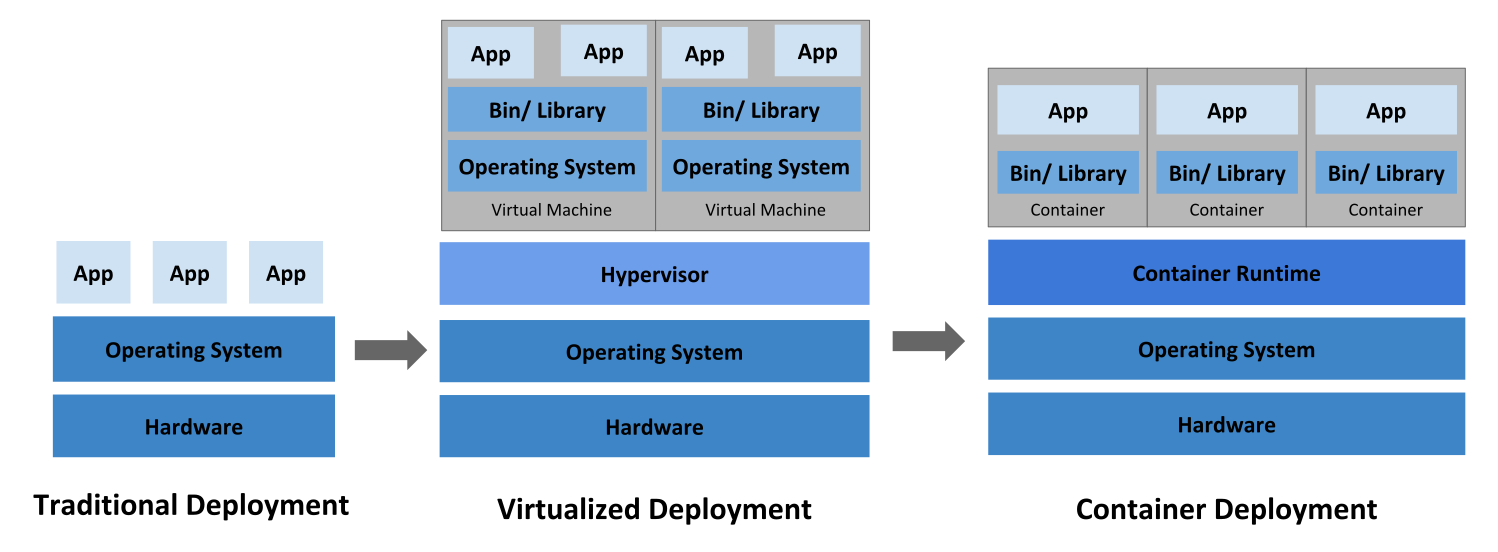
\includegraphics[width=\textwidth]{./imgs/container_evolution.png}
	\captionsource{Evolution of application deployment.}{https://kubernetes.io/docs/concepts/overview/what-is-kubernetes/}
	\label{fig:container-evolution}
\end{figure}

Containers can be thought of as lightweight virtual machines. Unlike the
latter, containers share the same kernel with the host machine but still allow
for a very controlled environment to run applications. There are many
benefits to this : separating the development from deployment, portability,
easy resource allocation, breaking large services into smaller micro-services
or support of continuous integration tools (containers greatly facilitate
integration tests).\\

The \textit{Cloud Native Computing Foundation (CNCF)
}\footnote{\url{https://www.cncf.io/}} was founded in the intent of leveraging
the container technology for an overall better web. In a general way, we now
speak of these containerized and modular applications as cloud native computing
:

\textit{``Cloud native technologies empower organizations to build and run
	scalable applications in modern, dynamic environments such as public,
	private, and hybrid clouds. Containers, service meshes, microservices,
	immutable infrastructure, and declarative APIs exemplify this
	approach.}

\textit{These techniques enable loosely coupled systems that
	are resilient, manageable, and observable.  Combined with robust
	automation, they allow engineers to make high-impact changes frequently
	and predictably with minimal toil.``}\footnote{\url{https://github.com/cncf/toc/blob/master/DEFINITION.md}}

Kubernetes\footnote{\url{https://kubernetes.io/}} is the implementation of this
general idea and was announced at the same time as the CNCF. It aims at
automating the administration of a fleet of containers. Deployment and scaling
(that is to say, replication of one same application to increase its
availability) is described in yaml files and managed by Kubernetes.  It is
industry grade and is now the de-facto solution for container orchestration.

\subsection{HPC and Kubernetes}

In this work we use Kubernetes schedulers as batch schedulers because batch
scheduling is our domain of origin (Batsim was developed in close relation with
	the teams behind the grid computing simulator
	SimGrid\cite{casanova:hal-01017319} and the resource manager OAR
\cite{oar}), and because it is convenient for us to test our approach with HPC
workloads. However, even though Kubernetes does have means to handle such
workloads like batch schedulers \cite{kube-batch} and a special type of
resource\footnote{https://kubernetes.io/docs/concepts/workloads/controllers/job/},
these two fields differ fundamentally because of the nature of the issues they
tackle. We do not intend to evaluate scheduler performance but rather prove
that such studies are possible with Batsim, which is why this work is conducted
this way. Still, there are perspectives for Kubernetes in the HPC community and
we believe HPC systems could benefit from this work.

The difference between HPC and cloud computing lies in the workloads they are
intended to tackle.  Kubernetes was designed to run applications. Services or
micro services are run in containers and are expected to be available at all
times : they are replicated as many times as desired and restarted whenever a
failure occurs. High availability is at the core of Kubernetes container
management.  On the other hand, depending on implemented scheduling policies,
HPC is focused on metrics such as user wait time, resource usage or energy
cost. One example of a fundamental difference between cluster computing and
batch scheduling is the handling of a task failure. In HPC it is sometimes not
sufficient to restart the single job that failed and the entire submission must
be re-run if it is part of several jobs computed in parallel. In cluster
computing the task is simply restarted without any other consideration -- other
than ensuring its dependencies are restarted with it.

Kubernetes is now the standard for AI and Machine Learning as shown by the many
efforts at making this coupling an efficient
environment\cite{lee2017design}\cite{233001}\cite{10.1145/3154842.3154845},
which brought an increasing interest for container driven HPC aswell and
Kubernetes for HPC in particular. Batch schedulers such as
kube-batch\footnote{\url{https://github.com/kubernetes-sigs/kube-batch}} have
been implemented for kube, and numerous HPC applications like
slurm\footnote{\url{https://slurm.schedmd.com/containers.html}} now support containers as well.

Indeed, containers have many advantages from which HPC users could benefit
from.
\begin{itemize}
	\item First off, research has shown that Kuberenetes offer similar
		performance to more standard bare metal HPC\cite{8950981}.
	\item Users will get the same environment everywhere making up for a
		uniform and standardized workplace.
	\item Portability : users could seamlessly hop from one infrastructure
		to another based on their needs and criteria like price,
		performance, and capabilities rather than compatibility.
	\item Encapsulation : HPC applications often rely on complex
		dependencies that can be easily concealed into containers.
\end{itemize}
%\begin{figure}[h]
%	\centering
%	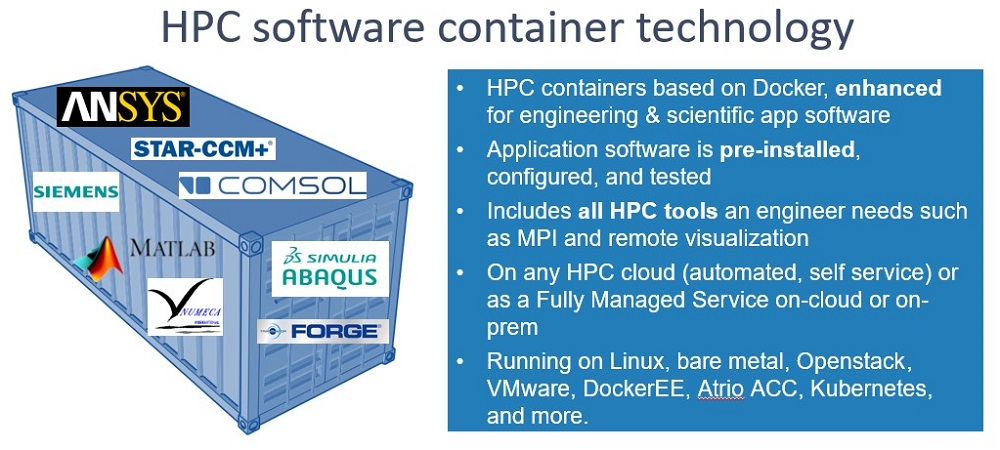
\includegraphics[scale=0.5]{./imgs/hpc-container.jpg}
%	\captionsource{The container technology for HPC}{https://www.hpcwire.com/2019/09/19/kubernetes-containers-and-hpc/}
%	\label{fig:hpc-container}
%\end{figure}

Despite all those advantages, Kubernetes is not ready yet to be used in proper
HPC environment because it lacks vital components like a proper batch job
queuing system and support for MPI applications. It cannot yet compete against
the very well established HPC ecosystem, but that time may come soon as
containers are becoming more and more integrated in modern infrastructures.

\section{Related work}

Not many projects exist on Kubernetes simulation or have been disclosed. We
were able to find two projects that propose simulations of Kubernetes clusters.

JoySim \cite{joysim} is a fully fledged Kubernetes simulator developed in an
industrial context. Simulations are based on synthetic events and their mock
nodes simply simulate a resource usage. The strength of this simulator is its
scalability which it obtains thanks to its very light weight simulated nodes.
JoySim is aimed at studying the quality of the scheduling and its performance
in complex scenarios by generating metrics such as resource usage and
scheduling time. Although, to the best of our knowledge, it is not suited for
batch scheduling and tackles more classic issues for Kubernetes such as
services availability and resource utilization.  The user may specify events to
occur during the simulation in order to test out different scenarios.
Unfortunately, while an open source released in planned, this piece of software
is currently closed source.

k8s-cluster-simulator \cite{k8s-cluster-simulator} is an open source cluster
simulator for evaluating schedulers, which originated from a end of studies
project like this work. Like JoySim, it relies on simple models: pods are
submitted with certain resource requirements, for a certain amount of time. One
can provide any scheduler implementation they want as long as they do so
through their Go interface. This reduces the amount of schedulers that can be
tested to Go implementations only, unless the user is willing to
implement an adaptive layer to support other schedulers.\\

Two simulators are very close to Batsim in terms of capabilities and
objectives, that is to say the study on scheduling policies.

Alea2\cite{alea2} is a grid computer system simulator based on GridSim. It is
therefore written in Java and cross platform. Like Batsim, its
\textit{ready-to-use} philosophy allow experimenting with different scheduling
policies with little set up overhead.  Alea2 strength lies in its modularity:
its object oriented paradigms make it very easily extensible and customizable.
Unlike Batsim it does not offer a decoupling of the simulator and the decision
process and therefore the user will have to rely on the implemented scheduling
algorithms, although these algorithms cover the most standardly used scheduling
policies.  The user will have to implement other policies he would like to test
out. The simulator handles inputs in the form of \textit{Standard Workloads
Format (SWF)} or \textit{Grid Workloads Format (GWF)}. Batsim proposes a script
to process SWF files into its own input format but does not handle them
directly.

Accasim\cite{10.1007/978-3-319-73353-1_12} is a simulator for studying
\textit{Workload Management Systems (WMS)} in HPC infrastructure. It is similar
to Alea in the sense that the decision process is not decoupled from the
simulator and standard scheduling algorithms are implemented in Accasim, so
that the user does not need to set up extra software in order to start
experimenting. In addition, the user may provide extra data about the system
status (power consumption, temperature or resource failures) in order to
support advanced scheduling algorithms.  These take the form of additional
events transmitted to the simulator. Accasim loads jobs incrementally and
cleans them upon completion which reduces its memory usage compared to Batsim,
which loads everything in memory at the start of the simulation.

What truly distinguishes Batsim from these simulators is the strong decoupling
between the RJMS and the simulator, which allows us to experiment with RJMS
software rather than only studying scheduling policies. This allows us to
evaluate the scheduler computing needs or memory usage independently, as if it
was running in real conditions. Performance wise, we cannot really compare
Batsim with Alea and Accasim contrary to what is stated in
\cite{10.1007/978-3-319-73353-1_12}.  Indeed, this study was realized with SWF
workloads which can only depict delays. This is adapted to Accasim and Alea
because their models are simple, but not to SimGrid models which are too
advanced for this type of workload.  These simulators are not comparable
because of the fundamental differences in their models.

%NOTES
%
%Simulators are often intentionally very specialized. Some are aimed at specific
%domains like peer-to-peer computing simulators like PeerSim
%\cite{p2p09-peersim} and OverSim \cite{baumgart2009oversim}, or volunteer
%computing simulators (\cite{simBA}, \cite{alonso2017combos})
%
%Simulators based on simgrid: 
%
%Problems with simulation: often unrealeased simulators, or designed for a
%specific project, or short lived (OptorSim)
%
%Simulators specific to platforms: YARNSim, SLURM simulator\footnote{https://github.com/ubccr-slurm-simulator/slurm\_simulator} 
%
%Exemples of papers with custom unreleased simulators: \cite{yabuuchi2019lowlatency} by the same guys who made kubernetes-simulator.\\
%
%list of simulators
%\begin{itemize}
%	\item SimGrid, GridSim, CloudSim, GroudSim (to cite the most important).
%	\item Other simulators in unrelated domains: SimBA (volunteer computing), PeerSim, OverSim (peer to peer), WRENCH (workflows).
%	\item HPC simulation: off-line vs on-line
%	\item Interconnected networks Simulation: INSEE (environment for interconnected networks), SICOSYS. Aimed to be used with other tools like SIMICS to extend th ecapabilities.
%	\item Low level simulation: SIMICS, RSIM and SimOS (multiprocessor systems).
%	\item discontinued/old projects: GSSIM, Simbatch
%\end{itemize}
%
%Kubernetes simulation: k8-cluster-simulator, joySim.
